\chapter{الترسيب والذوبانية}\label{ch:b1:precipitation}

تسقط قطرة من نترات الفضة في ماء الصنبور فتظهر سحابة بيضاء:
إنها كلوريد الفضة، المتكوّن من الملّيغرامات القليلة من أيونات الكلوريد في كل
لتر. والماء المتسرب عبر الحجر الجيري يحمل كربونات الكالسيوم ثم
يرسّبها من جديد، جزءًا من الملّيمتر كل سنة، على هيئة
الصواعد والنوازل في المغارات. وحصاة الكلية راسب أيضًا. وكل من هذه
توازن بين جسم صلب وأيوناته في المحلول، وثابت
واحد، هو \omterm{def:b1:precipitation:solubility-product}{جداء الذوبانية}، يقول هل يتكوّن الجسم الصلب، وكم
يذوب منه، وكيف تتغير ذوبانيته حين يتغير أيون آخر أو
pH. وبه يستطيع الكيميائي أن يفصل الأيونات بعضها عن بعض
بترسيبها الواحد تلو الآخر --- وهذا أساس معالجة مياه المناجم
التي يُختم بها هذا الفصل.

\begin{recall}
قاس المجلد المدرسي (الصفان السادس والثاني عشر) \omterm{def:b1:precipitation:solubility}{الذوبانية} بالغرام لكل
لتر وتعرّف الأيونات بالرواسب التي تعطيها. وقد وُضع ثابت
التوازن \omterm{def:b1:extent-q-and-k:quotient}{وخارج التفاعل} $Q$ والنشاطيات (1 للجسم الصلب النقي
أو للمذيب، و$c/c^\circ$ للمذاب) في
\cref{ch:b1:extent-q-and-k}: يمضي التفاعل في الاتجاه المباشر ما دام $Q < K$. أما
طريقة \omterm{def:b1:predominant-reaction:predominant-reaction}{التفاعل الغالب} وسلّم $\mathrm{p}K_a$ فمصدرهما
\cref{ch:b1:predominant-reaction}؛ ولا يُكتب $c^\circ = \qty{1}{mol/L}$
في الخوارج.
\end{recall}

\begin{omfigure}
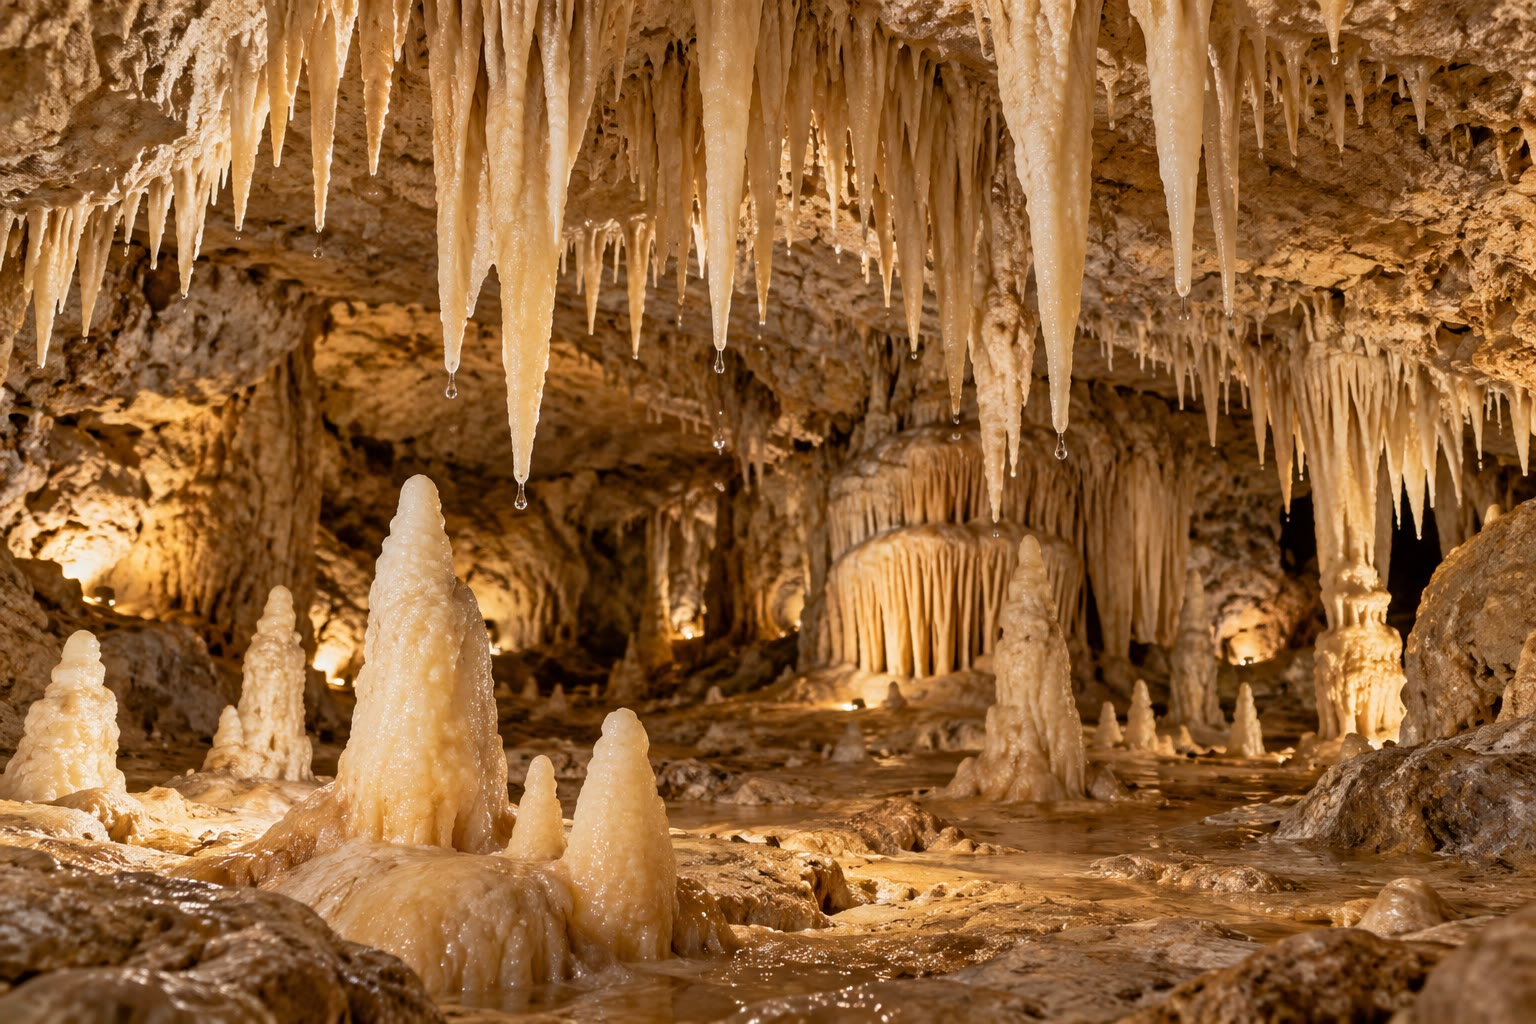
\includegraphics[width=0.62\linewidth]{images/book2/ai/b1-11-cave.jpg}

{\small نوازل وصواعد في مغارة كلسية. يذيب الماء الغني
بثنائي أكسيد الكربون كربونات الكالسيوم في التربة فوقها؛ وفي المغارة
يفقد جزءًا من ثنائي أكسيد الكربون فتترسب الكربونات من جديد
(\cref{exo:b1:precipitation:10}).}
\end{omfigure}

\section{جداء الذوبانية}\label{sec:b1:precipitation:product}

تفقد \omterm{def:b1:crystals-metals:crystal}{بلورة} من كلوريد الفضة تُلقى في الماء أيونات لصالح
المحلول، ويعيد المحلول بعضها إلى \omterm{def:b1:crystals-metals:crystal}{البلورة}. وحين تتساوى
السرعتان يكون المحلول \emph{مشبعًا}: لا يعود تركيبه
يتغير، مع أن الأيونات تظل تنتقل في الاتجاهين
(الشكل أدناه).

\begin{definition}[جداء الذوبانية]\label{def:b1:precipitation:solubility-product}
\emph{جداء الذوبانية}\index{جداء الذوبانية} $K_s$ لجسم صلب
أيوني $\mathrm{M}_a\mathrm{X}_b$ هو ثابت توازن
ذوبانه إلى أيوناته،
\[
  \mathrm{M}_a\mathrm{X}_b\mathrm{(s)} \rightleftharpoons a\,\mathrm{M}^{m+}
  + b\,\mathrm{X}^{x-}, \qquad
  K_s = [\mathrm{M}^{m+}]_{\mathrm{eq}}^{\,a}\,[\mathrm{X}^{x-}]_{\mathrm{eq}}^{\,b},
  \qquad \mathrm{p}K_s = -\log K_s ,
\]
إذ \omterm{def:b1:extent-q-and-k:activity}{نشاطية} الجسم الصلب 1. وهو، ككل ثابت توازن، لا يتعلق
إلا بدرجة الحرارة.
\end{definition}

من أجل كلوريد الفضة، \ce{AgCl(s) <=> Ag+ + Cl-} و$K_s =
[\ce{Ag+}][\ce{Cl-}] = 10^{-9.75}$؛ ومن أجل فلوريد الكالسيوم، \ce{CaF2(s) <=>
Ca^2+ + 2F-} و$K_s = [\ce{Ca^2+}][\ce{F-}]^2 = 10^{-9.84}$؛ ومن أجل
هيدروكسيد الحديد(III)، $K_s = [\ce{Fe^3+}][\ce{OH-}]^3 = 10^{-38.55}$.
ويسرد الجدول أدناه القيم المستعملة في هذا المجلد.
وهي محسوبة، مثل قيم $\mathrm{p}K_a$ في
\cref{ch:b1:predominant-reaction}، من طاقات غيبس القياسية المجدولة
للتكوين: $\mathrm{p}K_s = \Delta_r G^\circ/(RT\ln 10)$، وهي علاقة
تُستخرج في مجلد السنة الثانية.

\begin{omfigure}
\begin{tikzpicture}[font=\small, >={Stealth}]
  % the crystal: alternating Ag+ (small, grey) and Cl- (large, green)
  \foreach \i in {0,1,2,3,4,5}
    \foreach \j in {0,1,2} {
      \pgfmathtruncatemacro{\pp}{mod(\i+\j,2)}
      \ifnum\pp=0
        \shade[ball color=green!55!black!60] (\i*0.62,\j*0.62) circle (0.29);
      \else
        \shade[ball color=gray!35] (\i*0.62,\j*0.62) circle (0.17);
      \fi }
  \draw[thick, gray] (-0.45,-0.45) rectangle (3.55,1.75);
  \node[below] at (1.55,-0.45) {\ce{AgCl(s)}};
  % ions in solution
  \shade[ball color=gray!35] (1.2,3.0) circle (0.17);
  \node[right] at (1.4,3.0) {\ce{Ag+}};
  \shade[ball color=green!55!black!60] (2.6,2.7) circle (0.29);
  \node[right] at (2.9,2.7) {\ce{Cl-}};
  \shade[ball color=gray!35] (4.4,1.4) circle (0.17);
  \shade[ball color=green!55!black!60] (5.1,2.6) circle (0.29);
  \shade[ball color=gray!35] (-1.0,2.4) circle (0.17);
  \shade[ball color=green!55!black!60] (-0.6,3.3) circle (0.29);
  % arrows: dissolution and precipitation
  \draw[->, thick, omDef] (1.24,1.6) to[bend left=20] node[left, pos=0.6] {ذوبان} (1.15,2.78);
  \draw[->, thick, omProp] (2.55,2.38) to[bend left=20] node[right, pos=0.45] {ترسيب} (2.45,1.55);
  % the water line
  \draw[blue!50, thick] (-1.6,3.8) -- (5.9,3.8);
  \node[blue!60!black, anchor=east] at (5.9,4.05) {محلول مشبع};
\end{tikzpicture}

{\small \omterm{def:b1:crystals-metals:crystal}{بلورة} من كلوريد الفضة في محلولها المشبع. تغادر أيونات
السطح (الذوبان) وتُأسر أخرى (الترسيب) بالسرعة
نفسها، فيبقى $[\ce{Ag+}][\ce{Cl-}]$ مساويًا للثابت $K_s$. وقد رُسمت أيونات الفضة
أصغر من أيونات الكلوريد، كما هي في الواقع.}
\end{omfigure}

\begin{omfigure}
\begin{tabular}{lc@{\qquad}lc}
\hline
الجسم الصلب & $\mathrm{p}K_s$ & الجسم الصلب & $\mathrm{p}K_s$ \\
\hline
\ce{AgCl} & 9.75 & \ce{Ca(OH)2} & 5.33 \\
\ce{AgBr} & 12.27 & \ce{Mg(OH)2} & 11.25 \\
\ce{AgI} & 16.07 & \ce{Fe(OH)2} & 16.31 \\
\ce{Ag2CrO4} & 11.95 & \ce{Zn(OH)2} & 16.38 \\
\ce{BaSO4} & 9.97 & \ce{Fe(OH)3} & 38.55 \\
\ce{CaCO3} (الكالسيت) & 8.30 & \ce{Al(OH)3} (الجبسيت) & 34.75 \\
\ce{CaF2} & 9.84 & & \\
\hline
\end{tabular}

\smallskip
{\small \omterm{def:b1:precipitation:solubility-product}{جداءات الذوبانية} عند \qty{25}{\celsius}، محسوبة من
طاقات غيبس القياسية لتكوين الأجسام الصلبة والأيونات
المائية. وثوابت التكوين المستعملة في هذا الفصل (\cref{sec:b1:precipitation:amphoteric}):
$\log\beta_4 = 14.45$ للأيون \ce{Zn(OH)4^2-}، و33.52 للأيون \ce{Al(OH)4-}،
و$\log\beta_1 = 11.82$ للأيون \ce{FeOH^2+}.}
% ledger: dfg:AgCl_cr, dfg:AgBr_cr, dfg:AgI_cr, dfg:Ag2CrO4_cr, dfg:Ag+_ao, dfg:Cl-_ao, dfg:Br-_ao, dfg:I-_ao, dfg:CrO42-_ao (computed in figdata/bachelor-1/aqueous-constants.py)
% ledger: dfg:BaSO4_cr, dfg:Ba2+_ao, dfg:SO42-_ao, dfg:CaCO3_cr, dfg:CO32-_ao, dfg:CaF2_cr, dfg:Ca2+_ao, dfg:F-_ao (computed, same script)
% ledger: dfg:Ca_OH2_cr, dfg:Mg_OH2_cr, dfg:Mg2+_ao, dfg:Fe_OH2_cr, dfg:Fe2+_ao, dfg:Zn_OH2_cr, dfg:Zn2+_ao, dfg:Fe_OH3_cr, dfg:Fe3+_ao, dfg:Al2O3.3H2O_cr, dfg:Al3+_ao, dfg:OH-_ao (computed, same script)
% ledger: dfg:Zn_OH42-_ao, dfg:Al_OH4-_ao, dfg:FeOH2+_ao (formation constants, same script)
\end{omfigure}

\begin{proposition}[شرط الترسيب]\label{prop:b1:precipitation:precipitation-condition}
ليحوِ محلول أيونات جسم صلب $\mathrm{M}_a\mathrm{X}_b$،
\omterm{def:b1:extent-q-and-k:quotient}{وخارج تفاعل} الذوبان فيه $Q_s = [\mathrm{M}^{m+}]^a[\mathrm{X}^{x-}]^b$.
\begin{itemize}
  \item إذا كان $Q_s < K_s$، فلا يمكن أن يكون الجسم الصلب حاضرًا عند التوازن:
        المحلول غير مشبع وكل جسم صلب يضاف يذوب، كليًا
        إن لم يكن كثيرًا.
  \item إذا كان $Q_s > K_s$، ترسّب الجسم الصلب حتى يصير $Q_s = K_s$.
  \item لا يتعايش الجسم الصلب والمحلول في \omterm{def:b1:extent-q-and-k:quantitative}{حالة توازن} إلا حين
        $Q_s = K_s$.
\end{itemize}
\end{proposition}

\begin{proof}
وفق \cref{ch:b1:extent-q-and-k}، يمضي الذوبان في الاتجاه المباشر ما دام
$Q_s < K_s$ وفي الاتجاه العكسي (الترسيب) ما دام $Q_s > K_s$. وما دام
الذوبان يمضي مباشرًا فإن $Q_s$ يتزايد. فإن نفد الجسم الصلب قبل أن
يبلغ $Q_s$ القيمة $K_s$، توقف التطور ولم يبقَ جسم صلب: فالتفاعل
الذي يشارك فيه \omterm{def:b1:extent-q-and-k:system}{طور} مكثف نقي يمكن أن يتوقف قبل التوازن لأن
كمية ذلك \omterm{def:b1:extent-q-and-k:system}{الطور} لا يمكن أن تصير سالبة. وإذا كان $Q_s > K_s$، خفّض الترسيب
تركيزي الأيونين كليهما وتناقص $Q_s$ حتى يساوي $K_s$،
وهذا ممكن دائمًا، لأن الأيونات موجودة.
\end{proof}

والنقطة الأخيرة هي ما يميز الجسم الصلب من النوع المذاب. فالنوع
الحمضي--القاعدي حاضر عند كل pH، مهما قلّ؛ أما الجسم الصلب فإما
حاضر وإما غائب. ولهذا يكون مخططه مخطط
\emph{وجود}، لا \omterm{def:b1:predominant-reaction:predominance}{مخطط غلبة}
(\cref{sec:b1:precipitation:domains}).

\begin{example}[خلط محلولين]\label{ex:b1:precipitation:mixing}
يُخلط \qty{10.0}{mL} من نترات الفضة تركيزها \qty{2.0e-4}{mol/L} مع
\qty{10.0}{mL} من كلوريد الصوديوم تركيزه \qty{2.0e-4}{mol/L}. وبعد
الخلط مباشرة، وقبل أي تفاعل، $[\ce{Ag+}] = [\ce{Cl-}] = \qty{1.0e-4}{mol/L}$
و$Q_s = 10^{-8.0} > K_s = 10^{-9.75}$: فيترسب كلوريد الفضة.
ومع المحلولين كليهما بتركيز \qty{2.0e-6}{mol/L}، يكون $Q_s = 10^{-12.0} < K_s$
ويبقى الخليط رائقًا. فنترات الفضة اختبار حساس لأيونات
الكلوريد، لكنه ليس حساسًا بلا حدود.
\end{example}

\begin{inthelab}[اختبار الكلوريد]
في مختبر التعليم تضاف بضع قطرات من محلول نترات الفضة
إلى العيّنة، بعد تحميضها بحمض النتريك المخفف. فالحمض
يحوّل أيونات الكربونات والهيدروكسيد إلى ثنائي أكسيد الكربون وماء، وكانت
لولا ذلك ستترسب هي أيضًا مع أيونات الفضة. والراسب الأبيض
الذي يسودّ في الضوء هو كلوريد الفضة؛ ويعطي البروميد راسبًا
بلون القشدة ويعطي اليوديد راسبًا أصفر
(الصورة أدناه).
ونترات الفضة تُسوّد الجلد: فتُلبس القفازات والنظارات الواقية.
\end{inthelab}

\begin{omfigure}
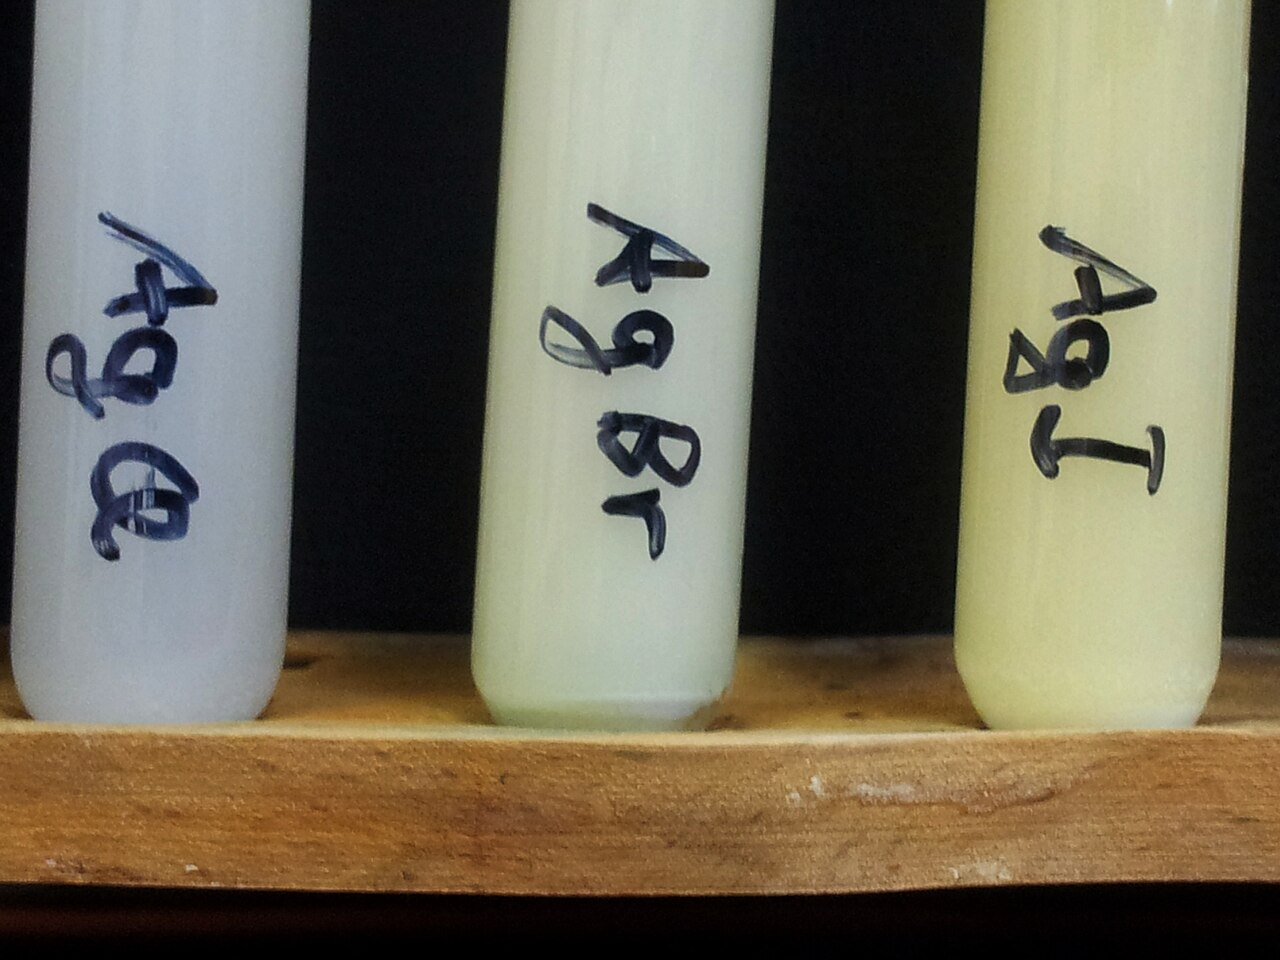
\includegraphics[width=0.6\linewidth]{images/book2/silver-halides.jpg}

{\small رواسب كلوريد الفضة (أبيض)، وبروميد الفضة (بلون القشدة)
ويوديد الفضة (أصفر باهت). تصوير رراوش1974، CC BY-SA 3.0،
ويكيميديا كومنز.}
\end{omfigure}

\section{الذوبانية}

\begin{definition}[الذوبانية]\label{def:b1:precipitation:solubility}
\emph{ذوبانية}\index{ذوبانية} $s$ جسم صلب في محلول معطى
هي كمية الجسم الصلب التي تذوب في لتر واحد من ذلك المحلول
حتى الإشباع (بالوحدة \unit{mol/L})؛ وإذا ضُربت في الكتلة المولية كانت
الذوبانية الكتلية، بالوحدة \unit{g/L}. وهي تتعلق بدرجة الحرارة
وبتركيب المحلول.
\end{definition}

\begin{proposition}[الذوبانية انطلاقًا من جداء الذوبانية]\label{prop:b1:precipitation:s-of-ks}
في الماء النقي، إذا لم تشارك الأيونات في أي تفاعل آخر،
\[
  \mathrm{MX}:\ s = \sqrt{K_s}, \qquad
  \mathrm{MX_2}\ \text{أو}\ \mathrm{M_2X}:\ s = \left(\frac{K_s}{4}\right)^{1/3},
  \qquad
  \mathrm{M}_a\mathrm{X}_b:\ s = \left(\frac{K_s}{a^a b^b}\right)^{1/(a+b)} .
\]
\end{proposition}

\begin{proof}
حين يذوب $s$ مول من الجسم الصلب في كل لتر، يكون $[\mathrm{M}^{m+}] = as$
و$[\mathrm{X}^{x-}] = bs$، فعند الإشباع $K_s = (as)^a(bs)^b =
a^a b^b s^{a+b}$. ومن أجل MX، $a = b = 1$؛ ومن أجل \ce{MX2}، $1^1 2^2 = 4$،
وكذلك من أجل \ce{M2X}.
\end{proof}

\begin{example}[كلوريد الفضة وكرومات الفضة]\label{ex:b1:precipitation:agcl-ag2cro4}
كلوريد الفضة: $s = 10^{-9.75/2} = \qty{1.3e-5}{mol/L}$، أي
\qty{1.9}{mg/L} مع $M = \qty{143.4}{g/mol}$. وكرومات الفضة \ce{Ag2CrO4}
($\mathrm{p}K_s = 11.95$): $s = (10^{-11.95}/4)^{1/3} =
\qty{6.6e-5}{mol/L}$. فللكرومات $K_s$ أصغر، ومع ذلك فهي أذوب
بخمس مرات. ولا تُقارن \omterm{def:b1:precipitation:solubility-product}{جداءات الذوبانية} مباشرة إلا
بين أجسام صلبة من نمط الصيغة نفسه.
\end{example}

\begin{remark}
تفترض الصيغ أن الأيونات حرة. ففي الماء النقي أيون الكرومات
\omterm{def:b1:predominant-reaction:strong-acid}{قاعدة ضعيفة} وأيون الفضة لا يعقّده شيء، فتكون
النتيجة قريبة من الصواب في كرومات الفضة؛ أما في الكربونات أو
الكبريتيد أو الهيدروكسيد فخواص الأنيون القاعدية مهمة ويلزم
القسم التالي. وعند شدة أيونية عالية تبتعد النشاطيات أيضًا
عن التراكيز، وهو تصحيح متروك لمجلد السنة الثانية.
\end{remark}

\section{أثر الأيون المشترك وأثر pH}

\begin{definition}[أثر الأيون المشترك]\label{def:b1:precipitation:common-ion}
\emph{أثر الأيون المشترك}\index{أثر الأيون المشترك} هو انخفاض
\omterm{def:b1:precipitation:solubility}{ذوبانية} جسم صلب في محلول يحوي أصلًا أحد
أيوناته.
\end{definition}

\begin{proposition}[الذوبانية مع أيون مشترك]\label{prop:b1:precipitation:common-ion}
ليذُب MX في محلول فيه أصلًا $[\mathrm{X}^-] = c$، مع
$c \gg \sqrt{K_s}$. عندئذ $s \approx K_s/c$، وهي أصغر بكثير منها في الماء
النقي. ومن أجل \ce{MX2} في محلول يحوي \ce{M^2+} بتركيز $c$،
$s \approx \frac12\sqrt{K_s/c}$.
\end{proposition}

\begin{proof}
عند الإشباع $[\mathrm{M}^+] = s$ و$[\mathrm{X}^-] = c + s$، فيكون
$s(c + s) = K_s$. وإذا كان $s \ll c$، فإن $s = K_s/c$؛ والفرض صحيح لأن
$K_s/c \ll c$ حين $c^2 \gg K_s$. ومن أجل \ce{MX2}، $[\ce{X-}] = 2s$
و$[\mathrm{M}^{2+}] = c + s \approx c$، فيكون $c\,(2s)^2 = K_s$.
\end{proof}

كلوريد الفضة في كلوريد الصوديوم تركيزه \qty{0.10}{mol/L}: $s = 10^{-9.75}/0.10
= \qty{1.8e-9}{mol/L}$، أي أقل بسبعة آلاف مرة منها في الماء. ولهذا
يُغسل الراسب بمحلول مخفف لأيون مشترك بدلًا من
الماء النقي: فيفقد منه أقل.

وحين يكون أنيون الجسم الصلب قاعدة، ينتزعه الحمض من
توازن الذوبان فتزداد \omterm{def:b1:precipitation:solubility}{الذوبانية}. ومن أجل كربونات الكالسيوم في
الحمض،
\[
  \ce{CaCO3(s) + H3O+ <=> Ca^2+ + HCO3- + H2O}, \qquad
  K = \frac{K_s}{K_{a2}} = 10^{-8.30 + 10.33} = 10^{2.03} ,
\]
وهو تفاعل مواتٍ: فالخل أو حمض الكلوريدريك يذيب الحجر الجيري،
وثنائي أكسيد الكربون المتكوّن من تفاعل
\ce{HCO3-} اللاحق يعطي الفوران المألوف.
% ledger: dfg:HCO3-_ao (pKa2 of carbonic acid, ch. 10)

\begin{proposition}[ذوبانية هيدروكسيد بدلالة pH]\label{prop:b1:precipitation:hydroxide-ph}
في محلول منظَّم عند pH معطى، يخضع تركيز \ce{M^{n+}}
المتوازن مع الهيدروكسيد \ce{M(OH)_n} للعلاقة
\[
  \log[\mathrm{M}^{n+}] = -\mathrm{p}K_s + n\,(\mathrm{p}K_e - \mathrm{pH}) ,
\]
وهي مستقيم ميله $-n$ بدلالة pH. وإذا لم يكوّن الأيون أي معقد،
كانت هذه \omterm{def:b1:precipitation:solubility}{ذوبانية} الهيدروكسيد.
\end{proposition}

\begin{proof}
$K_s = [\mathrm{M}^{n+}][\ce{OH-}]^n$ و$[\ce{OH-}] = K_e/[\ce{H3O+}]$،
فيكون $\log[\mathrm{M}^{n+}] = \log K_s - n\log[\ce{OH-}] = -\mathrm{p}K_s -
n(\mathrm{pH} - \mathrm{p}K_e)$.
\end{proof}

فكل وحدة pH تقسم \omterm{def:b1:precipitation:solubility}{ذوبانية} هيدروكسيد الحديد(III) على
ألف، \omterm{def:b1:precipitation:solubility}{وذوبانية} هيدروكسيد الزنك على مئة. فالهيدروكسيدات
تُرسَّب، وتُذاب من جديد، بتغيير pH.

\begin{example}[إذابة كربونات الكالسيوم بثنائي أكسيد الكربون]\label{ex:b1:precipitation:cave}
الماء الذي يحوي ثنائي أكسيد الكربون مذابًا يذيب الكالسيت:
\[
  \ce{CaCO3(s) + CO2(aq) + H2O <=> Ca^2+ + 2HCO3-}, \qquad
  K = \frac{K_s K_{a1}}{K_{a2}} = 10^{-8.30 - 6.37 + 10.33} = 10^{-4.34} ,
\]
والثابت مستخرج بجمع ذوبان الكربونات،
والحمضية الأولى لثنائي أكسيد الكربون، وعكس الحمضية الثانية. وكلما
كثر ثنائي أكسيد الكربون ذاب من كربونات الكالسيوم أكثر. وهواء التربة عادةً
أغنى بكثير بثنائي أكسيد الكربون من هواء المغارة؛ فالماء الذي
عبر التربة وبلغ سقف المغارة يفقد ثنائي أكسيد الكربون،
ويترسب الكالسيت (\cref{exo:b1:precipitation:10}).
\end{example}

\section{مناطق الوجود والترسيب الانتقائي}\label{sec:b1:precipitation:domains}

\begin{definition}[منطقة الوجود]\label{def:b1:precipitation:existence-domain}
من أجل جسم صلب وتركيز كلي معطى $c$ لأحد أيوناته، تكون
\emph{منطقة وجود}\index{منطقة الوجود} الجسم الصلب هي مجال
المتغير (pX أو pM أو pH) الذي يكون فيه الجسم الصلب حاضرًا عند
التوازن. وحدّها هو القيمة التي تظهر عندها أول حبيبة من الجسم
الصلب، حين $Q_s = K_s$ والأيون لا يزال بالتركيز $c$.
\end{definition}

\begin{method}[رسم مخطط وجود]\label{met:b1:precipitation:existence-domain}
\begin{enumerate}
  \item ثبّت التركيز الكلي $c$ للأيون غير الوارد على
        المحور (مثلًا $[\ce{Ag+}]_{\mathrm{tot}} = c$ على محور pCl).
  \item اكتب $K_s$ عند بدء الترسيب، والأيون لا يزال عند
        $c$، وحلّ بالنسبة إلى المتغير الوارد على المحور.
  \item يوجد الجسم الصلب في الجهة التي يكون فيها الأيون الآخر
        مركّزًا: pCl صغير (كلوريد كثير)، أو pAg صغير، أو pH عالٍ
        في الهيدروكسيد.
  \item لا تعلّم منطقة للأيون نفسه: فهو حاضر
        في كل مكان، بالتركيز $c$ خارج منطقة الجسم الصلب وبأقل من $c$
        داخلها.
\end{enumerate}
\end{method}

من أجل كلوريد الفضة مع $c = [\ce{Ag+}]_{\mathrm{tot}} = 10^{-2}$:
يبدأ الترسيب حين $[\ce{Cl-}] = K_s/c = 10^{-7.75}$، فيوجد الجسم الصلب
من أجل $\mathrm{pCl} < 7.75$. ومن أجل يوديد الفضة يقع الحد عند
$\mathrm{pI} = 16.07 - 2 = 14.07$، كما هو مرسوم أدناه.

\begin{omfigure}
\begin{tikzpicture}[font=\small, >={Stealth}, x=0.62cm]
  \fill[omDef!18] (0,0.12) rectangle (7.75,0.6);
  \draw[->, thick] (0,0) -- (17.2,0) node[right] {\foreignlanguage{arabic}{\babelsublr{pCl} أو \babelsublr{pI}}};
  \foreach \x in {0,2,4,6,8,10,12,14,16}
    \draw (\x,0.08) -- (\x,-0.08) node[below] {\x};
  \draw[omDef, thick] (7.75,-0.5) -- (7.75,0.9);
  \node[omDef] at (3.9,0.36) {\foreignlanguage{arabic}{\ce{AgCl(s)} موجود}};
  \node[omDef, above] at (7.75,0.9) {7.75};
  \node[anchor=west] at (8.0,0.36) {\foreignlanguage{arabic}{لا جسم صلب: \ce{Ag+} بتركيز $10^{-2}$ \babelsublr{mol/L}}};
  % AgI below
  \begin{scope}[yshift=-1.9cm]
  \fill[omProp!20] (0,0.12) rectangle (14.07,0.6);
  \draw[->, thick] (0,0) -- (17.2,0);
  \foreach \x in {0,2,4,6,8,10,12,14,16}
    \draw (\x,0.08) -- (\x,-0.08) node[below] {\x};
  \draw[omProp, thick] (14.07,-0.5) -- (14.07,0.9);
  \node[omProp] at (7.0,0.36) {\foreignlanguage{arabic}{\ce{AgI(s)} موجود}};
  \node[omProp, above] at (14.07,0.9) {14.07};
  \end{scope}
\end{tikzpicture}

{\small منطقتا وجود كلوريد الفضة (على محور pCl، في الأعلى)
ويوديد الفضة (على محور pI، في الأسفل) من أجل تركيز كلي للفضة
قدره \qty{1.0e-2}{mol/L}. فاليوديد يرسّب الفضة عند تراكيز
أدنى بمليون مرة مما يفعل الكلوريد.}
\end{omfigure}

\begin{method}[الترسيب الانتقائي]\label{met:b1:precipitation:selective}
لفصل أيونين يترسبان بالكاشف نفسه:
\begin{enumerate}
  \item احسب، لكل أيون عند تركيزه، تركيز الكاشف
        (أو pH) الذي يبدأ عنده تكوّن جسمه الصلب؛ فالأدنى
        يترسب أولًا؛
  \item احسب تركيز الأيون الأول الباقي في المحلول حين
        يبدأ الثاني بالترسيب؛
  \item يكون الفصل مقبولًا إذا كان ذلك التركيز كسرًا صغيرًا
        بما يكفي من التركيز الابتدائي --- \qty{0.1}{\percent} عادةً
        --- ويوقَف عندئذ إضافة الكاشف بين العتبتين.
\end{enumerate}
\end{method}

\begin{example}[اليوديد والكلوريد]\label{ex:b1:precipitation:i-cl}
يحوي محلول أيونات اليوديد والكلوريد، كلاهما بتركيز
\qty{1.0e-2}{mol/L}؛ وتضاف نترات الفضة قطرة قطرة، دون
تخفيف. يبدأ يوديد الفضة بالتكوّن عند $[\ce{Ag+}] = 10^{-16.07 + 2} =
10^{-14.07}$، وكلوريد الفضة عند $10^{-9.75 + 2} = 10^{-7.75}$: فاليوديد
يترسب أولًا. وحين يظهر كلوريد الفضة، يكون
$[\ce{I-}] = 10^{-16.07}/10^{-7.75} = 10^{-8.32} = \qty{4.8e-9}{mol/L}$،
أي كسرًا $5 \times 10^{-7}$ من اليوديد: فالفصل تام.
\end{example}

وتُفصل الهيدروكسيدات بالطريقة نفسها والمتغير هو pH.
ويبيّن المخطط أدناه، لستة أيونات تركيز كل منها
\qty{0.010}{mol/L}، قيمة pH التي يظهر عندها الهيدروكسيد وقيمة pH التي يكون
قد ترسب عندها \qty{99.9}{\percent} من الأيون. فالحديد(III) والألومنيوم
يُزالان في الماء الحمضي، والزنك والحديد(II) قرب التعادل، والمغنيسيوم
حول pH 10، والكالسيوم في الماء الشديد القاعدية فقط.

\begin{omfigure}
\begin{tikzpicture}
\begin{axis}[
  width=0.82\linewidth, height=5.4cm, xmin=0, xmax=14, ymin=0.4, ymax=6.6,
  axis x line=bottom, axis y line=left, xlabel={\babelsublr{pH}},
  xtick={0,2,4,6,8,10,12,14}, ytick={1,2,3,4,5,6},
  yticklabels={\ce{Fe^3+}, \ce{Al^3+}, \ce{Zn^2+}, \ce{Fe^2+}, \ce{Mg^2+}, \ce{Ca^2+}},
  y dir=reverse, axis line style={-},
  tick label style={font=\small}, label style={font=\small}]
\addplot[draw=none, omDef!35,
  error bars/.cd, x dir=plus, x explicit,
  error bar style={line width=7pt, omDef!35}, error mark=none]
  table[x=start, y=row, x error expr=14-\thisrow{start}] {figdata/out/bachelor-1-solubility-ph-thresholds.dat};
\addplot[draw=none, omDef,
  error bars/.cd, x dir=plus, x explicit,
  error bar style={line width=7pt, omDef}, error mark=none]
  table[x=start, y=row, x error expr=\thisrow{end}-\thisrow{start}] {figdata/out/bachelor-1-solubility-ph-thresholds.dat};
\end{axis}
\end{tikzpicture}

{\small ترسيب الهيدروكسيدات من محاليل تركيز كل
أيون فيها \qty{0.010}{mol/L}. يمتد الشريط الداكن من أول حبيبة هيدروكسيد إلى قيمة pH
التي يكون عندها \qty{99.9}{\percent} من الأيون قد ترسب (بعرض وحدة pH واحدة
للأيون الثلاثي التكافؤ، ووحدة ونصف للثنائي التكافؤ)؛ والشريط الفاتح هو
بقية \omterm{def:b1:precipitation:existence-domain}{منطقة وجود} الهيدروكسيد. ولم تُبيَّن إعادة الذوبان
المذبذبة لهيدروكسيدي الزنك والألومنيوم عند pH العالي
(\cref{sec:b1:precipitation:amphoteric}).}
\end{omfigure}

\section{الهيدروكسيدات المذبذبة}\label{sec:b1:precipitation:amphoteric}

أضف هيدروكسيد الصوديوم قطرة قطرة إلى محلول كبريتات الزنك: يتكوّن راسب
أبيض من هيدروكسيد الزنك، ثم يذوب من جديد في الهيدروكسيد
المفرط. ويفعل هيدروكسيد الألومنيوم الشيء نفسه؛ أما هيدروكسيدا الحديد(III)
والمغنيسيوم فلا.

\begin{definition}[الهيدروكسيد المذبذب]\label{def:b1:precipitation:amphoteric-hydroxide}
يكون الهيدروكسيد \emph{هيدروكسيدًا مذبذبًا}\index{هيدروكسيد مذبذب}
إذا ذاب في الحمض، على هيئة الكاتيون، وفي القاعدة المفرطة، على هيئة
أنيون معقد هيدروكسيلي:
\[
  \ce{Zn(OH)2(s) + 2H3O+ -> Zn^2+ + 4H2O}, \qquad
  \ce{Zn(OH)2(s) + 2OH- -> Zn(OH)4^2-} .
\]
\end{definition}

المعقدات وثوابتها موضوع \cref{ch:b1:complexation}؛ ونذكر منها هنا
الأنيون المعقد \ce{Zn(OH)4^2-}، أي رباعي هيدروكسو الزنكات، وثابت تكوينه
$\beta_4 = [\ce{Zn(OH)4^2-}]/([\ce{Zn^2+}][\ce{OH-}]^4)
= 10^{14.45}$.

\begin{proposition}[ذوبانية هيدروكسيد مذبذب]\label{prop:b1:precipitation:amphoteric}
إذا لم يوجد الزنك في المحلول إلا على هيئة \ce{Zn^2+} و\ce{Zn(OH)4^2-}، كانت
\omterm{def:b1:precipitation:solubility}{ذوبانية} هيدروكسيد الزنك
\[
  s = [\ce{Zn^2+}] + [\ce{Zn(OH)4^2-}] = \frac{K_s}{[\ce{OH-}]^2} + K\,[\ce{OH-}]^2,
  \qquad K = \beta_4 K_s = 10^{-1.93} .
\]
وفي تمثيل $\log s$ بدلالة pH يتبع مستقيمًا ميله $-2$ عند pH المنخفض ومستقيمًا
ميله $+2$ عند pH العالي. وتكون أصغر ما يمكن عند
$[\ce{OH-}]^4 = K_s/K = 1/\beta_4$، أي عند $\mathrm{pH} =
\mathrm{p}K_e - \frac14\log\beta_4$، حيث $s_{\min} = 2\sqrt{K_s K}$.
\end{proposition}

\begin{proof}
عند الإشباع $[\ce{Zn^2+}] = K_s/[\ce{OH-}]^2$،
و$[\ce{Zn(OH)4^2-}] = \beta_4[\ce{Zn^2+}][\ce{OH-}]^4 = \beta_4 K_s
[\ce{OH-}]^2$. ومع $w = [\ce{OH-}]^2$، تكون مشتقة $s(w) = K_s/w + Kw$ هي
$-K_s/w^2 + K$، المنعدمة عند $w = \sqrt{K_s/K}$، حيث $s = 2\sqrt{K_s K}$. وعند
pH المنخفض يغلب الحد الأول ويكون $\log s = \log K_s - 2\log[\ce{OH-}]$
(الميل $-2$ بدلالة pH)؛ وعند pH العالي يغلب الثاني، $\log s = \log K + 2\log[\ce{OH-}]$
(الميل $+2$).
\end{proof}

بالقيم أعلاه، تقع القيمة الصغرى عند $\mathrm{pH} = 14.00 - 14.45/4
= 10.39$ و$s_{\min} = 2 \times 10^{-(16.38 + 1.93)/2} =
\qty{1.4e-9}{mol/L}$
(الشكل أدناه). أما القيمة الصغرى
الحقيقية فأعلى بكثير: فالزنك يكوّن أيضًا \ce{ZnOH+} و\ce{Zn(OH)3-} و،
قبل كل شيء، \ce{Zn(OH)2(aq)} المذاب غير المشحون، الذي لا يتعلق تركيزه
المتوازن مع الجسم الصلب بقيمة pH. والحساب الكامل،
بالجداول نفسها، يضع الحد الأدنى قرب
$10^{-5.6}$~mol/L. فنموذج النوعين يعطي الميول وترتيب
العتبات؛ أما قرب القيمة الصغرى فكل نوع يُحسب له حساب.

\begin{omfigure}
\begin{tikzpicture}
\begin{axis}[name=zn,
  width=0.46\linewidth, height=5.6cm, xmin=6, xmax=14, ymin=-10, ymax=0,
  axis x line=bottom, axis y line=left, xlabel={\babelsublr{pH}}, ylabel={\babelsublr{$\log s$}},
  xtick={6,8,10,12,14}, ytick={-10,-8,-6,-4,-2,0},
  tick label style={font=\small}, label style={font=\small}]
\addplot[omProp, dashed, thick] table[x=pH, y=full] {figdata/out/bachelor-1-solubility-ph-zinc.dat};
\addplot[omDef, very thick] table[x=pH, y=model] {figdata/out/bachelor-1-solubility-ph-zinc.dat};
\node[font=\small, anchor=west] at (axis cs:7.0,-1.0) {\ce{Zn^2+}};
\node[font=\small, anchor=east] at (axis cs:13.8,-1.1) {\ce{Zn(OH)4^2-}};
\node[font=\small, omProp, anchor=south] at (axis cs:10.4,-5.5) {كل الأنواع};
\node[font=\small, anchor=north] at (axis cs:10.2,-0.4) {الزنك};
\end{axis}
\begin{axis}[at={(zn.east)}, anchor=west, xshift=1.8cm,
  width=0.46\linewidth, height=5.6cm, xmin=2, xmax=14, ymin=-10, ymax=0,
  axis x line=bottom, axis y line=left, xlabel={\babelsublr{pH}}, ylabel={\babelsublr{$\log s$}},
  xtick={2,4,6,8,10,12,14}, ytick={-10,-8,-6,-4,-2,0},
  tick label style={font=\small}, label style={font=\small}]
\addplot[omDef, very thick] table[x=pH, y=model] {figdata/out/bachelor-1-solubility-ph-aluminium.dat};
\node[font=\small, anchor=west] at (axis cs:3.4,-0.8) {\ce{Al^3+}};
\node[font=\small, anchor=east] at (axis cs:13.8,-0.6) {\ce{Al(OH)4-}};
\node[font=\small, anchor=north] at (axis cs:8.6,-0.4) {الألومنيوم};
\end{axis}
\end{tikzpicture}

{\small \omterm{def:b1:precipitation:solubility}{ذوبانية} هيدروكسيد الزنك (يسارًا) وهيدروكسيد الألومنيوم،
الجبسيت (يمينًا)، بدلالة pH، في نموذج النوعين (الخطوط المتصلة): الميلان
$-2$ و$+2$ للزنك، و$-3$ و$+1$ للألومنيوم. وفي الزنك يشمل المنحنى المتقطع كل
الأنواع الهيدروكسيلية، ويضع \ce{Zn(OH)2(aq)} غير المشحون حدًا أدنى.}
\end{omfigure}

وفي الألومنيوم يكون الهيدروكسيد \ce{Al(OH)3} والمعقد \ce{Al(OH)4-}،
فيكون \ce{Al(OH)3(s) + OH- <=> Al(OH)4-} مع $K = \beta_4 K_s = 10^{33.52
- 34.75} = 10^{-1.23}$ والميلان $-3$ و$+1$. ويُستعمل الفرق بين
الألومنيوم والحديد(III) --- أحدهما مذبذب والآخر لا --- في
الصناعة لفصلهما: فهيدروكسيد الصوديوم الساخن يذيب
ألومنيوم البوكسيت ويترك أكاسيد الحديد خلفه
(\cref{exo:b1:precipitation:12}).

\section{تمارين}

\begin{exercise}[$\star$]\label{exo:b1:precipitation:1}
اكتب معادلة الذوبان وعبارة $K_s$ لكل من
\ce{BaSO4} و\ce{CaF2} و\ce{Ag2CrO4} و\ce{Fe(OH)3}. وأعطِ $K_s$ بقوى
العشرة من الجدول الوارد في \cref{sec:b1:precipitation:product}، و$\mathrm{p}K_s$
لجسم صلب جداء ذوبانيته $K_s = \num{2.0e-13}$.
\end{exercise}

\begin{exercise}[$\star$]\label{exo:b1:precipitation:2}
احسب \omterm{def:b1:precipitation:solubility}{ذوبانية} بروميد الفضة في الماء النقي بالوحدة \unit{mol/L}
وبالوحدة \unit{mg/L} ($M = \qty{187.8}{g/mol}$).
\end{exercise}

\begin{exercise}[$\star$]\label{exo:b1:precipitation:3}
يُخلط \qty{50}{mL} من كلوريد الباريوم تركيزه \qty{2.0e-3}{mol/L} مع
\qty{50}{mL} من كبريتات الصوديوم تركيزها \qty{2.0e-4}{mol/L}. هل تترسب
كبريتات الباريوم؟ السؤال نفسه مع كبريتات الصوديوم بتركيز
\qty{2.0e-7}{mol/L}.
\end{exercise}

\begin{exercise}[$\star$]\label{exo:b1:precipitation:4}
احسب \omterm{def:b1:precipitation:solubility}{ذوبانية} كبريتات الباريوم في الماء النقي، ثم في
محلول كبريتات الصوديوم تركيزه \qty{0.010}{mol/L}. بأي عامل
تغيرت؟
\end{exercise}

\begin{exercise}[$\star\star$]\label{exo:b1:precipitation:5}
احسب \omterm{def:b1:precipitation:solubility}{ذوبانية} فلوريد الكالسيوم في الماء النقي (بالوحدة \unit{mol/L}
و\unit{mg/L}، $M = \qty{78.1}{g/mol}$)، ثم في محلول كلوريد
الكالسيوم تركيزه \qty{0.10}{mol/L}. تحقق من التقريب الذي أجريته.
\end{exercise}

\begin{exercise}[$\star\star$]\label{exo:b1:precipitation:6}
يحوي محلول أيونات المغنيسيوم بتركيز \qty{0.050}{mol/L}. عند أي pH يبدأ
هيدروكسيد المغنيسيوم بالترسيب؟ وعند أي pH يكون \qty{99}{\percent} من
المغنيسيوم قد ترسب؟ ارسم \omterm{def:b1:precipitation:existence-domain}{منطقة وجود} \ce{Mg(OH)2} على
محور pH.
\end{exercise}

\begin{exercise}[$\star\star$]\label{exo:b1:precipitation:7}
يحوي محلول أيونات البروميد والكلوريد، كلاهما بتركيز
\qty{1.0e-2}{mol/L}. وتضاف نترات الفضة دون تخفيف. أي
راسب يظهر أولًا؟ وما كسر الأيون الأول الذي لا يزال في
المحلول حين يظهر الجسم الصلب الثاني؟ هل الفصل مقبول؟
\end{exercise}

\begin{exercise}[$\star\star$]\label{exo:b1:precipitation:8}
تستعمل معايرة مور للكلوريد بأيونات الفضة أيونات الكرومات
كاشفًا: إذ يجب ألا تظهر كرومات الفضة الحمراء إلا حين يكون الكلوريد
قد ترسب كله تقريبًا. تركيز الكلوريد \qty{0.050}{mol/L} وتركيز الكرومات
\qty{5.0e-3}{mol/L}؛ ويُهمل التخفيف. احسب $[\ce{Ag+}]$ حين
تبدأ كرومات الفضة بالتكوّن، وكسر الكلوريد الذي لا يزال في
المحلول في تلك اللحظة.
\end{exercise}

\begin{exercise}[$\star\star$]\label{exo:b1:precipitation:9}
تُرجّ كربونات الكالسيوم مع محلول يبقيه \omterm{def:b1:predominant-reaction:buffer}{محلول منظم} عند pH 8.30،
حيث الهيدروجينوكربونات هي إلى حد بعيد نوع الكربونات الرئيسي. بيّن أن
$[\ce{Ca^2+}][\ce{HCO3-}] = K_s\,10^{\mathrm{p}K_{a2} - \mathrm{pH}}$،
واحسب \omterm{def:b1:precipitation:solubility}{الذوبانية}، بافتراض أن كل الكربونات المذابة تبقى
على هيئة \ce{HCO3-} ($\mathrm{p}K_{a2} = 10.33$).
\end{exercise}

\begin{exercise}[$\star\star\star$]\label{exo:b1:precipitation:10}
المغارات الكلسية. تتبع \omterm{def:b1:precipitation:solubility}{ذوبانية} ثنائي أكسيد الكربون التوازن
\ce{CO2(g) <=> CO2(aq)} مع $\log K_H = -1.47$ ($K_H =
[\ce{CO2(aq)}]/p(\ce{CO2})$، والضغط بالبار).
\begin{enumerate}
  \item اجمع $K_H$ مع الثابت الوارد في
        \cref{ex:b1:precipitation:cave} لتحصل على ثابت
        \ce{CaCO3(s) + CO2(g) + H2O <=> Ca^2+ + 2HCO3-}.
  \item بيّن أن \omterm{def:b1:precipitation:solubility}{ذوبانية} الكالسيت هي $s = (K'p/4)^{1/3}$
        واحسبها في ماء توازن مع هواء التربة عند
        $p(\ce{CO2}) = \qty{0.010}{bar}$، ثم مع الهواء الطلق،
        \qty{4.26e-4}{bar}. وأعطِ الاثنتين بالوحدة \unit{mg/L} من \ce{CaCO3}
        ($M = \qty{100.1}{g/mol}$).
  \item فسّر نمو النازلة.
\end{enumerate}
\end{exercise}

\begin{exercise}[$\star\star\star$]\label{exo:b1:precipitation:11}
يُرفع pH محلول للزنك تركيزه \qty{1.0e-2}{mol/L} تدريجيًا،
ولا يوجد الزنك إلا على هيئة \ce{Zn^2+} و\ce{Zn(OH)4^2-}.
\begin{enumerate}
  \item بين أي قيمتين من قيم pH يكون هيدروكسيد الزنك حاضرًا؟
  \item أوجد pH الذي تكون عنده \omterm{def:b1:precipitation:solubility}{الذوبانية} أصغر ما يمكن، \omterm{def:b1:precipitation:solubility}{والذوبانية} الصغرى.
  \item ارسم إجمالًا $\log s$ بدلالة pH وعلّم الميول.
\end{enumerate}
\end{exercise}

\begin{exercise}[$\star\star\star$]\label{exo:b1:precipitation:12}
يحوي محلول أيونات الألومنيوم والحديد(III)، تركيز كل منها
\qty{1.0e-3}{mol/L}. ويضاف هيدروكسيد الصوديوم بإفراط.
\begin{enumerate}
  \item فوق أي pH يكون كل الألومنيوم مذابًا على هيئة \ce{Al(OH)4-}؟
  \item كم يكون عندئذ تركيز \ce{Fe^3+}؟ واستنتج ما يتعلق
        بالفصل.
  \item فسّر لماذا يخفق الفصل لو وُضع المغنيسيوم مكان
        الألومنيوم.
\end{enumerate}
\end{exercise}

\section{مسألة: تنظيف مياه منجم}

\begin{problem}[{مسألة نهاية الأسبوع --- عتبات ترسيب ثلاثة
هيدروكسيدات، والمعقد الهيدروكسيلي للحديد(III)، واسترجاع الزنك
وإعادة ذوبانه المذبذبة، ونافذة pH لإزالة الحديد(III)
دون فقد الزنك \babelsublr{(II)}}]
\label{pb:b1:precipitation:1}
الماء المتسرب من منجم فلزات قديم حمضي (pH 2.0) ويحوي
الحديد(III) بتركيز \qty{1.0e-3}{mol/L}، والزنك(II) بتركيز \qty{5.0e-3}{mol/L}
والمغنيسيوم بتركيز \qty{2.0e-2}{mol/L}. وترفع المحطة pH خطوة خطوة
لتزيل الحديد حمأةً نفايةً، ثم لتسترجع الزنك على هيئة
هيدروكسيده، تاركةً المغنيسيوم غير الضار في الماء. معطيات عند
\qty{25}{\celsius}: $\mathrm{p}K_s$ للمركب \ce{Fe(OH)3} 38.55، وللمركب \ce{Zn(OH)2}
16.38، وللمركب \ce{Mg(OH)2} 11.25؛ $\log\beta_4(\ce{Zn(OH)4^2-}) = 14.45$؛
$\log\beta_1(\ce{FeOH^2+}) = 11.82$؛ $\mathrm{p}K_e = 14.00$؛ والكتل المولية:
\ce{Fe(OH)3} \qty{106.8}{g/mol}، \ce{Zn(OH)2} \qty{99.4}{g/mol}.

\medskip
\noindent\textbf{الجزء الأول --- أي هيدروكسيد أولًا؟}
\begin{enumerate}
  \item اكتب توازنات ذوبان الهيدروكسيدات الثلاثة
        و$K_s$ كل منها.
  \item فسّر لماذا لا تكفي قيم $\mathrm{p}K_s$ الثلاث وحدها لمعرفة أي
        هيدروكسيد يترسب أولًا.
  \item بيّن أن \ce{M(OH)_n} يبدأ بالترسيب من محلول
        \ce{M^{n+}} تركيزه $c$ عند $\mathrm{pH} = \mathrm{p}K_e -
        \frac1n(\mathrm{p}K_s + \log c)$.
  \item احسب قيمة pH هذه للحديد(III).
  \item احسبها للزنك.
  \item احسبها للمغنيسيوم.
  \item أعطِ ترتيب الترسيب مع ارتفاع pH. هل يترسب
        شيء في المياه عند خروجها من المنجم؟
\end{enumerate}

\medskip
\noindent\textbf{الجزء الثاني --- إزالة الحديد: تقدير أول.}
\begin{enumerate}[resume]
  \item تريد المحطة إخراج \qty{99.9}{\percent} من الحديد من الماء. فما
        تركيز الحديد المذاب الذي يسمح به ذلك؟
  \item بإهمال أي معقد، عند أي pH يُبلغ ذلك؟
  \item بيّن أنه في \omterm{def:b1:precipitation:existence-domain}{منطقة وجود} \ce{Fe(OH)3} يتناقص
        $\log[\ce{Fe^3+}]$ بمقدار 3 لكل وحدة pH.
  \item حتى أي pH يبقى الزنك كله في المحلول؟
  \item أعطِ التقدير الأول لنافذة pH التي يُزال فيها الحديد
        بينما يبقى الزنك.
\end{enumerate}

\medskip
\noindent\textbf{الجزء الثالث --- المعقد الهيدروكسيلي للحديد(III).}
\begin{enumerate}[resume]
  \item اكتب تكوّن \ce{FeOH^2+} من \ce{Fe^3+} و\ce{OH-}،
        وثابته.
  \item ارسم \omterm{def:b1:predominant-reaction:predominance}{مخطط الغلبة} للنوعين \ce{Fe^3+} و\ce{FeOH^2+}
        بدلالة pH.
  \item عند pH المستخرج في السؤال 9، احسب
        $[\ce{FeOH^2+}]/[\ce{Fe^3+}]$. هل كان التقدير الأول مأمونًا؟
  \item عبّر عن الحديد المذاب الكلي $[\ce{Fe^3+}] + [\ce{FeOH^2+}]$
        المتوازن مع \ce{Fe(OH)3} دالةً في pH.
  \item بيّن أن لوغاريتم \ce{FeOH^2+}، حيث يغلب هذا النوع،
        يتناقص بمقدار 2 لكل وحدة pH.
  \item أوجد pH الذي يهبط عنده الحديد المذاب الكلي إلى القيمة
        المستخرجة في السؤال 8.
\end{enumerate}

\medskip
\noindent\textbf{الجزء الرابع --- استرجاع الزنك.}
\begin{enumerate}[resume]
  \item بعد ترشيح حمأة الحديد يُرفع pH من جديد. عند
        أي pH يكون \qty{99}{\percent} من الزنك قد ترسب؟ وهل يتكوّن هيدروكسيد
        المغنيسيوم عند هذا pH؟
  \item اكتب تفاعل هيدروكسيد الزنك مع أيونات الهيدروكسيد المفرطة
        واحسب ثابته.
  \item فوق أي pH يعود الزنك كله إلى المحلول؟ وماذا يعني
        ذلك للمشغّل؟
  \item احسب كتلة حمأة هيدروكسيد الحديد(III) المزالة لكل متر
        مكعب من المياه.
  \item احسب كتلة هيدروكسيد الزنك المسترجعة لكل متر مكعب عند
        pH السؤال 19.
  \item لماذا يجب إزالة الحديد قبل الزنك، لا إزالتهما
        معًا؟
  \item اذكر نافذة pH، بمنزلتين عشريتين، التي يُزال فيها الحديد(III)
        بنسبة \qty{99.9}{\percent} بينما يبقى الزنك(II) كله في
        المحلول.
\end{enumerate}
\end{problem}
